\section{Převodníky sigma-delta}
- základní zapojení a funkce, příklady využití.

Základní koncepce převodníků sigma-delta
\begin{itemize}
\item převzorkování měřeného signálu (oversampling) s převzorkovacím koeficientem OSR,
\item tvarování šumového signálu za účelem dalšího potlačení (noise-shaping) a zvýšení SNR a tím i zvýšení počtu bitů,
\item číslicová filtrace (digital filtering),
\item decimace.
\end{itemize}

Blok H(z) je integrátor, který se chová jako diskrétní filtr. Kvantovací obvod generuje digitální výstup y[k], který je tvořen součtem výstupu integrátoru y\textsubscript{h}[k] a kvantovací chyby e\textsubscript{q}[k]. Diskrétní filtr je obtížné analyzovat díky nelineárnímu chování kvantovacího obvodu. Jednou z metod, jak dosáhnout použitelných výsledků, je
nahrazení skutečného kvantovacího obvodu jeho lineárním modelem. Tato linearizace je použita k vysvětlení funkce modulátoru sigma-delta. 
\begin{figure}[h]
   \begin{center}
     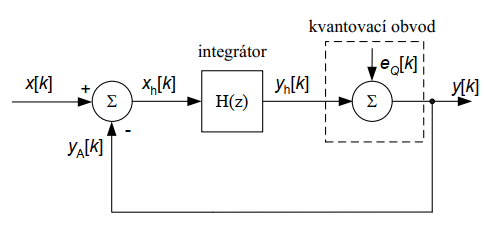
\includegraphics[scale=0.6]{images/sigma.png}
   \end{center}
   \caption{Blokové schéma lineárního modelu modulátoru sigma-delta}
\end{figure}

Signálová přenosová funkce (STF) a šumová přenosová funkce (NTF):
\begin{equation}
STF = \frac{H(z)}{1+H(z)}
\end{equation}

\begin{equation}
NTF = \frac{1}{1+H(z)}
\end{equation}

Jestliže je integrátor zvolen tak, že má mít vysoký zisk ve zpracovávaném pásmu f\textsubscript{B} a malý zisk mimo zpracovávané pásmo f\textsubscript{B}, pak se \textbf{STF} blíží 1 ve zpracovávaném pásmu. Mimo zpracovávané pásmo se STF blíží 0. 

Na druhou stranu, zisk \textbf{NTF} se blíží 0 ve zpracovávaném pásmu a 1 se blíží mimo zpracovávané pásmo. 

Diskrétní model integrátoru sigma-delta s jedním integrátorem je popisován jako modulátor sigma-delta prvního řádu. Zvyšováním řádu dochází k problému nestability modulátoru sigma-delta. Lineární model nemůže předpovídat, zda bude modulátor stabilní (nelze předpovídat, jestli póly reálného systému jsou uvnitř jednotkové kružnice = kritérium stability). V lineárním modelu je kvantovací obvod nahrazován jako konstantní zisk.
\begin{figure}[h]
   \begin{center}
     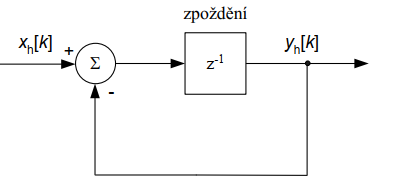
\includegraphics[scale=0.6]{images/sigma_dis.png}
   \end{center}
   \caption{Diskrétní model integrátoru}
\end{figure}

\pagebreak
U reálného kvantovacího obvodu je zisk proměnný. Přesnost
lineárního modelu se zvyšuje se zvyšujícím se rozlišení kvantovacího obvodu. Avšak jediná cesta jak dokázat, že je modulátor sigma-delta stabilní, je použití počítačové simulace.

Při návrhu modulátoru sigma-delta se volí optimální volbou mezi poměrem převzorkování (OSR), rozlišením kvantovacího obvodu N a řádem modulátoru sigma-delta k.

\subsection{Modulátory sigma-delta prvního řádu}
Na výstupu modulátoru sigma-delta je výstupní posloupnost bitů (bitstream). Bitstream je 1-bitový signál. Digitální 1 představuje nejvyšší možnou výstupní hodnotu a 0 představuje nejnižší možnou výstupní hodnotu. Kvantovací chyba v každém kroku je velká, protože je použit kvantovací obvod pouze se dvěma úrovněmi, průměruje kvantovaný signál, a proto se výstup modulátoru shoduje s analogovým vstupem. Tato střední hodnota je vypočítána decimačním filtrem, který následuje za modulátorem. Časová řada na výstupu integrátoru roste a klesá podle hodnoty zpětné vazby DAC. 1-bitový výstup z ADC je tvořen posloupností jedniček a nul, která modulováním šířky a periody impulzu reprezentuje vstupní analogovou hodnotu.
\begin{figure}[h]
   \begin{center}
     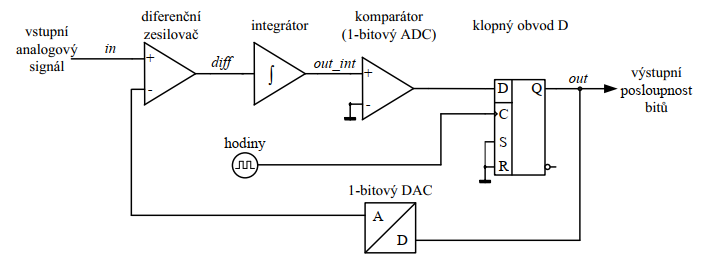
\includegraphics[scale=0.6]{images/sigmajedna.png}
   \end{center}
   \caption{Modulátor sigma-delta prvního řádu}
\end{figure}

Rozlišení modulátoru se zvyšuje s růstem počtu průměrovaných vzorků. To odpovídá růstu OSR. Na druhou stranu se snižuje šířka zpracovávaného pásma, a proto se musí volit kompromis mezi rozlišením a časem.

\subsection{Modulátory sigma-delta vyššího řádu}
Počet integrátorů v přímé větvi lze obecně libovolně zvyšovat, ale s tím narůstají problémy se stabilitou obvodu. Na případu jednoduché soustavy se zpětnou vazbou s více integrátory v přímé větvi si lze představit zdroj těchto problémů. Nestabilita modulátoru vyššího řádu nastane, pokud dojde k přetížení kvantovacího obvodu. Nestabilita nastává, když je vstup kvantovacího obvodu vybuzen vstupním signálem s vysokou amplitudou a nízkým kmitočtem.

Ve struktuře modulátoru sigma-delta jsou často používány integrátory se spínanými kapacitory a to ze dvou důvodů. Za prvé, přesnost koeficientů je určena poměrem kapacitorů, které je možné dosáhnout v technologii MOS s velkou přesností. Za druhé, hodnoty koeficientů nejsou závislé na vzorkovacím poměru, který je možné potom jednoduše změnit.
\begin{figure}[h]
   \begin{center}
     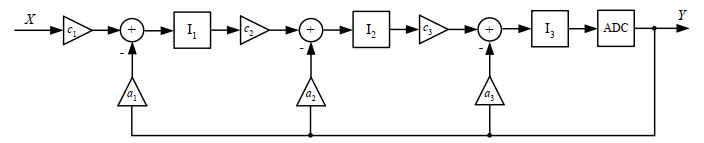
\includegraphics[scale=0.6]{images/sigmamulti.png}
   \end{center}
   \caption{Příklad modulátoru sigma-delta vyššího řádu}
\end{figure}

\subsection{Modulátory sigma-delta typu MASH}
U převodníků sigma-delta vyšších řádů byl velký problém se zajištěním stability celé soustavy. Řešením je paralelní zapojení jednoduchých modulátorů sigma-delta označováné jako převodník sigma-delta typu MASH (Multi Stage Noise Shaper).

\subsection{Sigma-delta převodník AD s filtrem typu pásmová propust}

Sigma-delta převodník AD s filtrem typu pásmová propust (bandpass filter) není tak známý jako jeho tradiční varianta, kdy je na výstupu připojen filtr typu dolní propust, nicméně jedná se o zapojení, které je poměrně často využíváno pro přímý převod komplexního analogového signálu na číslicový signál reprezentující amplitudu a fázi.

Tento typ převodníku je vhodný pro demodulaci kvadraturních, amplitudově modulovaných (QAM) signálů, tedy v GPS/GSM komunikačních systémů.

Bloková struktura modulátoru, která je tvořena bandpass filtrem, N-bitovým kvantovacím obvodem a číslicově-analogovým převodníkem zapojeným ve zpětné vazbě. Souvislost mezi kmitočtem vstupního signálu fin a hodinovým kmitočtem (f\textsubscript{s} = 4. fin) způsobuje, že je převodník fázově citlivý. Proto je nutné použít dva digitální filtry typu dolní propust Bandpass filtr lze syntetizovat pomocí kaskádního zapojení dvou nebo více bikvadraturních filtrů či rezonátorů, které musí mít ostrou převodní charakteristiku a jasně definovaný rezonanční kmitočet na kmitočtu f\textsubscript{n}. Tyto rezonátory lze implementovat jako diskrétní filtry využitím techniky spínaných kapacitorů nebo spínaných proudů.
\begin{figure}[h]
   \begin{center}
     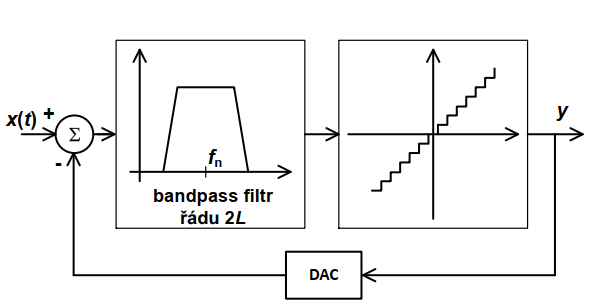
\includegraphics[scale=0.6]{images/sigmaBP.png}
   \end{center}
   \caption{Bloková struktura sigma-delta modulátoru s filtrem typu pásmová propust}
\end{figure}

\subsection{Převodníky DAC typu sigma-delta}
Tyto digitálně-analogové převodníky pracují na obdobném principu jako převodníky ADC typu $\Sigma$-$\Delta$. Blokové schéma obsahuje vstupní filtr, modulátor $\Sigma$-$\Delta$, jednobitový převodník DAC a výstupní antialiasingový analogový filtr. Ten vyhlazuje průběh výstupního signálu a odstraňuje nežádoucí vysokofrekvenční složky, které se do signálu dostaly vzorkováním a chybami digitálního řetězce.

\begin{figure}[h]
   \begin{center}
     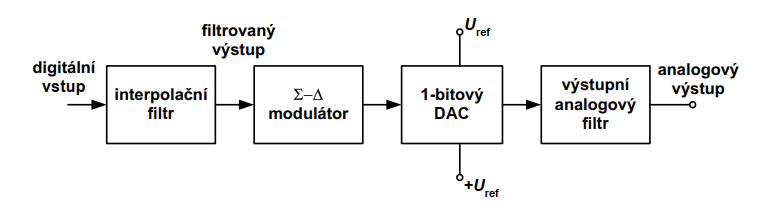
\includegraphics[scale=0.6]{images/sigmadac.png}
   \end{center}
   \caption{Příklad řešení převodníkem DAC typu $\Sigma$-$\Delta$}
\end{figure}

Rozdíl je však v implementaci. Vstupní filtr i modulátor $\Sigma$-$\Delta$ jsou digitální. Rozdíl
mezi hodnotami přicházejícího vzorku a číslicovou hodnotou reference (její polaritu řídí
vnitřní komparátor modulátoru) integrátor modulátoru integruje. Komparátor modulátoru
vyhodnocuje polaritu jeho výstupního signálu a podle ní ve vzorkovacích okamžicích připíná
na analogový výstup kladné nebo záporné analogové referenční napětí. Je-li vzorkování
dostatečně rychlé, odpovídá střední hodnota výstupního napětí digitální hodnotě vstupu. Zde
je nutné převzorkování. Čím přesnější má výstupní napětí být, tím je nutný delší interval pro
výpočet střední hodnoty, nebo tím vyšší musí být koeficient převzorkování.

Převzorkování společně s integrátorem modulátoru funguje jako antialiasingový filtr.
Ve výstupním řetězci je však signál číslicový a vstupní vzorky jsou k dispozici jen v určitých
okamžicích. Právě proto je tu vstupní digitální filtr výstupního řetězce (interpolační filtr).
Doplňuje ve vstupním proudu chybějící hodnoty, které jsou zapotřebí při převzokování.
Interpolační filtr dopočítává chybějící hodnoty pro převzorkování a odstraňuje tak ze
vstupního signálu všechny ty vysokofrekvenční složky, které se v digitální formě objevily digitalizací. Díky intermodulačnímu zkreslení a ještě dalším nelineárním zkreslením, se
mohou v použité části spektra objevit nepříjemné vedlejší efekty. Výstupní analogový filtr
vyhlazuje skokové změny analogového výstupu převodníku DAC. Bývá to analogový filtr
vyššího než druhého řádu.

\subsection{Decimační filtr}
V tradičních ADC pracující s Nyquistovým kmitočtem je kvantovací šum rozložen přes celé zpracovávané pásmo. Převodníky $\Sigma$-$\Delta$ pracují s pracovním kmitočtem několikanásobně vyšším než je Nyquistův kmitočet a kvantovací šum je rozložen do frekvenční oblasti přesahující rozsah zpracovávaného pásma
\begin{figure}[h]
   \begin{center}
     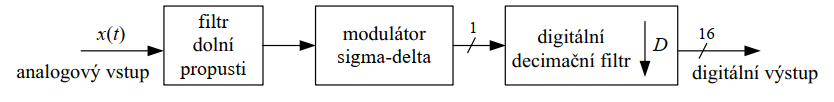
\includegraphics[scale=0.6]{images/sigmazak.png}
   \end{center}
   \caption{Základní systém převodníku sigma-delta}
\end{figure}

Díky filtraci výstupu modulátoru jsou tyto vysokofrekvenční složky odstraněny. Se vzrůstajícím řádem modulátoru dochází ke tvarování šumu, tak že kmitočtové spektrum je přesouváno do vyšších harmonických složek.

Funkcí decimačního filtru je odstranit šum z vyšších harmonických složek tak, aby nedošlo ke ztrátě signálu ve zpracovávaném pásmu. Další funkcí decimačního filtru je redukovat převzorkovaný výstupní signál modulátoru sigma-delta na signál s Nyquistovým kmitočtem. Návrh decimačního filtru závisí na digitálních koeficientech.
\newpage
\begin{figure}[h]
   \begin{center}
     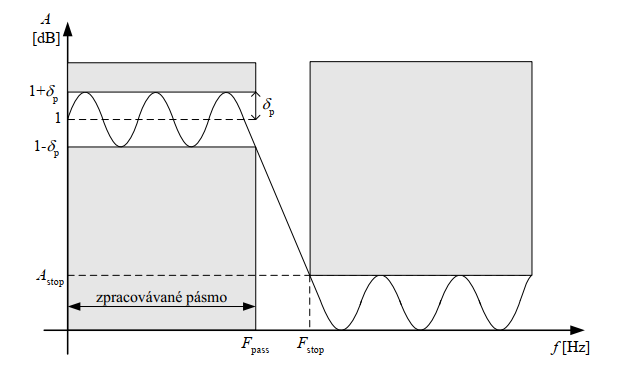
\includegraphics[scale=0.6]{images/decifiltr.png}
   \end{center}
   \caption{Kmitočtová charakteristika decimačního filtru}
\end{figure}

Kmitočet F\textsubscript{stop} je kmitočet, kdy dojde k zeslabení signálu na hodnotu A\textsubscript{stop}:
\begin{equation}
F_{stop}=\frac{F_{s}}{2*OSR}
\end{equation}






















